\section{Durchführung}
\label{sec:Durchführung}

Die für diesen Versuch verwendeeten Bauteile sind in \autoref{fig:Bauteile} dargestellt.
\begin{figure}[H]
    \centering
    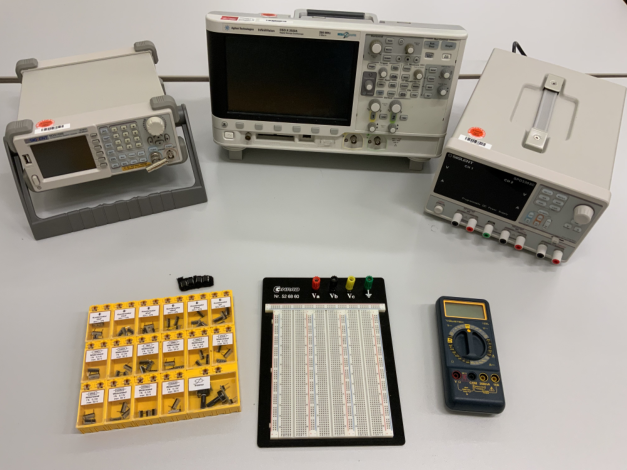
\includegraphics[width=0.4\linewidth]{figures/Aufbau.png}
    \caption{Für diesen Versuch benötigten Bauteile \cite{Anleitung51}.}
    \label{fig:Bauteile}
\end{figure}
\noindent
Als erstes wird die auf einem Steckbrett mithilfe eines LM741 Operationsverstärkers und der zur Verfügung stehenden Widerstände $R_1=\SI{1}{\kilo\ohm}$ und $R_2=\SI{100}{\kilo\ohm}$ ein invertierender Linearverstärker nach \autoref{fig:inverting-OpAmp} aufgebaut.
Von einem Frequenzgenerator wird eine Sinuspannung an den Eingang des Operationsverstärkers und an ein Oszilloskop angeschlossen.
Um die Abhängigkeit der Amplitude und der Phase zwischen Ein- und Ausgangsspannung von der Frequenz zu untersuchen, wird die Frequenz des Eingangssignals über mehrere Dekaden variiert und die Messwerte notiert.
Das Verhalten des OpAmps wird unter Verwendung verschiedener Widerstände wiederholt gemessen. \newline
Anschließend wird ein Integrator nach \autoref{fig:integrator} mit dem Widerstand $R=\SI{10}{\kilo\ohm}$ und $C=\SI{100}{\nano\farad}$ aufgebaut und der Frequenzgenerator wird auf eine Sinusspannung umgestellt.
Es wird erneut die Abhängigkeit der Amplitude und der Phase zwischen Ein- und Ausgangsspannung von der Frequenz untersucht.
Außerdem wird die Form der Ausgangsspannung bei einer Rechteck-, Sinus- und Dreieckspannung betrachtet, um das Integrationsverhalten des Schaltkreises zu überprüfen. \newline
In einer nachfolgenden Messung wird ein Differentiator nach \autoref{fig:Differentiator} mit dem Widerstand $R=\SI{100}{\kilo\ohm}$ und $C=\SI{22}{\nano\farad}$ aufgebaut.
Es werden die gleichen Messungen wie beim Integrator durchgeführt, um das Differentiationsverhalten des Schaltkreises zu überprüfen.
Im Gegensatz zum Integrator, werden allerdings hohe Frequenzen verwendet. \newline
Als nächstes wird die Schwellspannung eines Schmitt-Trigger nach \autoref{fig:Schmitt-Trigger} bestimmt, indem die Spannung stetig erhöht wird oder eine Dreieckspannung angelegt wird.
Die Schwellspannung wird mehrfach notiert und gemittelt. \newline
Zuletzt werden Generatoren untersucht, wofür zunächst ein Generator nach \autoref{fig:Generator_einzeln} aufgebaut wird.
Es werden die Widerstände $R_1=\SI{10}{\kilo\ohm}$, $R_2=\SI{100}{\kilo\ohm}$ und $R_3=\SI{1}{\kilo\ohm}$ und ein Kondensator mit der Kapazität $C=\SI{1}{\micro\farad}$ verwendet.
Um die Frequenz und die Amplitude des Generators zu bestimmen, wird die Ausgangsspannung an einem Oszilloskop gemessen. \newline
Zuletzt wird ein Generator mit variierender Amplitude nach \autoref{fig:Generator-varyingAmplitudes} mit $C=\SI{22}{\nano\farad}$ oder $C=\SI{100}{\nano\farad}$ aufgebaut und die Dämpfung der Amplitude und die Schwingungsdauer mithilfe eines Oszilloskopes aufgezeichnet.